\documentclass[a4paper,landscape]{article}
\def\micro{\mu m}
\def\um{$\micro$ }
\def\degreesC{$\degree$C }
\def\percent{$\%$ }

\usepackage{geometry}
	\geometry{a4paper,
	total={170mm,257mm},
	left=10mm,
	top=10mm,
	right=10mm,
	bottom=15mm,
}

../../global_color_scheme.tex
\usepackage[utf8]{inputenc}
\usepackage[english]{babel}
\usepackage{forloop}
\usepackage{array}
\usepackage{amsmath}
\usepackage{amsfonts}
\usepackage{amssymb}
\usepackage{gensymb}
\usepackage{mdframed}
\usepackage{graphicx}
\usepackage{tikz}
\usetikzlibrary{arrows,automata,shapes}
\usepackage[siunitx]{circuitikz}
\usepackage{makecell}
\usepackage{array}

\usepackage[colorlinks=true,linkcolor=blue,urlcolor=black,bookmarksopen=true]{hyperref}
\usepackage{bookmark}
\usepackage{hyperref}
\usepackage{sepfootnotes}
\usepackage{lipsum,tocloft} 
\usetikzlibrary{positioning}
\usetikzlibrary{patterns}

\usepackage{float}
\floatstyle{boxed} 
\restylefloat{figure}

\newcounter{TopProcessStep}
\newcounter{SubProcessStep}
\setcounter{TopProcessStep}{0}
\setcounter{SubProcessStep}{1}

\def\LastCleaniness{foo}

\newcommand{\getWaferCleaninessSymbol}[1]{
	\ifthenelse{\equal{#1}{clean}}{
\begin{tikzpicture}\node [fill=cyan, rounded corners=5pt] {Clean};\end{tikzpicture}} {
		\ifthenelse{\equal{#1}{semi-clean}} {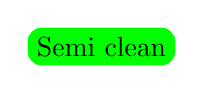
\begin{tikzpicture}\node [fill=green, rounded corners=5pt] {Semi clean};\end{tikzpicture}} {
			\ifthenelse{\equal{#1}{clean/semi-clean}} {
				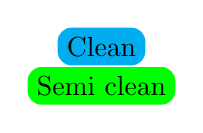
\begin{tikzpicture}
					\node [fill=cyan, rounded corners=5pt] at (0,0) {Clean};
					\node [fill=green, rounded corners=5pt] at (0,-0.5) {Semi clean};
				\end{tikzpicture}
			} {
				\ifthenelse{\equal{#1}{non-standard}} {
					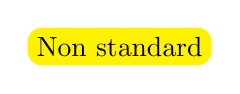
\begin{tikzpicture}
						\node [fill=yellow, rounded corners=5pt] {Non standard};
					\end{tikzpicture}} {undef}
			}
		}
	}
}

\newcommand{\makeProcessTable}[2]{
	\begin{tikzpicture}[node distance = 3cm, auto, thick,scale=0.3, every node/.style={transform shape}]
		\input{#1}
	\end{tikzpicture}
	\small\begin{tabular}{
		|>{\centering}p{1.5cm}
		|>{\centering}p{3cm}
		|>{\centering}p{1.5cm}
		|>{\centering}p{2cm}
		|>{\centering}p{4cm}
		|>{\centering}p{4cm}
		|>{\centering\arraybackslash\hspace{0pt}}p{2cm}|}
	\hline
	\textbf{Step Number} &
	\textbf{Equipment} &
	\textbf{Location} &
	\textbf{Cleanliness} &
	\textbf{Process} &
	\textbf{Requirements} &
	\textbf{Wafer Cleanliness}
	\setcounter{SubProcessStep}{1}
	\addtocounter{TopProcessStep}{1} \\
	\hline
	#2
	\end{tabular}
}

\newcommand{\addProcessStep}[6]{
\arabic{TopProcessStep}.\arabic{SubProcessStep}
\addtocounter{SubProcessStep}{1}
&
#1 &
#2 &
\getWaferCleaninessSymbol{#5} &
#3 &
#4 &
\getWaferCleaninessSymbol{#6} \\
\hline
}

\newcommand{\exposurePositiveStep}[1]{
	\addProcessStep{SVG Coater Track}{P200100}{HMDS, PR coating, soft bake}{AZ 504, 1.2µm, soft bake: 110C 1min}{clean/semi-clean}{clean}
	\addProcessStep{ASML Stepper}{P200100}{Exposure of the "#1" layer}{??}{clean/semi-clean}{clean}
	\addProcessStep{SVG Developer Track}{P200100}{Develop, Hard bake}{FHD-5, 1min; hard bake: 120C, 1min}{clean/semi-clean}{clean}
}

\newcommand{\exposureNegativeStep}[1]{
	\addProcessStep{SVG Coater Track}{P200100}{HMDS, PR coating, soft bake}{AZ 504, 1.2µm, soft bake: 110C 1min}{clean/semi-clean}{clean}
	\addProcessStep{ASML Stepper}{P200100}{Exposure of the "#1" layer}{??}{clean/semi-clean}{clean}
	\addProcessStep{SVG Developer Track}{P200100}{Develop, Hard bake}{FHD-5, 1min; hard bake: 120C, 1min}{clean/semi-clean}{clean}
}

\author{David Lanzendörfer}
\title{LibreSilicon process HKUST (NFF)}
\begin{document}
\maketitle

\begin{abstract}
	Copyright © 2017 LANCEVILLE TECHNOLOGY GROUP CO., LIMITED. All rights reserved. \\

This process is licensed under the Libre Silicon public license; you can redistribute it and/or modify it under the terms of the Libre Silicon public license
as published by the Libre Silicon alliance, either version 1 of the License, or (at your option) any later version.

This design is distributed in the hope that it will be useful, but WITHOUT ANY WARRANTY; without even the implied warranty of MERCHANTABILITY or FITNESS FOR A PARTICULAR PURPOSE.
See the Libre Silicon Public License for more details. \\

This document is part of the specification of the free silicon manufacturing standard for manufacturing the LibreSilicon standard logic cells\footnote{\url{https://git.libresilicon.com/?p=redmine/standard-cell-lib.git;a=summary}} and related free technology nodes from the LibreSilicon project.

For this initial revision 0.1 a gate-first approach has been chosen which led to the choice of polysilicon as the gate electrode material because of the simplicity of the gate alignment.
For better isolation properties of the transistors and gates in overall a box-isolation approach has been chosen.
All of these choices have been made with the future scale down from the recent $1 \mu m$ to smaller structure sizes.
\textbf{This process is for manufacturing $1 \mu m$ only!}
But further releases which will have been tested with smaller structure sizes can be expected.
 \\
	Please see the document with the generic steps\footnote{\url{https://github.com/leviathanch/libresiliconprocess/raw/master/process_steps/process_steps.pdf}}
	in order to get a detailed description of the different steps.	
\end{abstract}
\vfill
\newpage

Process Flow of Lanceville Technologies LibreSilicon 180nm

\begin{itemize}
	\item Project: LibreSilicon 1\um
	\item Name: Lanceville Technologies Group
	\item Substrate: P-Substrate silicon wafer <100>
	\item Date: \today
\end{itemize}

\begin{mdframed}[linewidth=2pt,linecolor=black]
\begin{center}
	\begin{tikzpicture}[node distance = 3cm, auto, thick,scale=1.0, every node/.style={transform shape}]
		% substrate
\fill[YellowOrange] (0,0) rectangle (20,2);
\node at (2,0.5) {Si (p-type)};
% n-well
\fill[Goldenrod] (1.25,0.75) rectangle (8.25,2);
\node at (5.75,1) {N-Well};
% body
\fill[ProcessBlue] (1.5,1) rectangle (3,2);
\node at (2,1.5) {n+};
% source
\fill[RedOrange] (3.5,1) rectangle (5,2);
\node at (4,1.5) {p+};
% drain
\fill[RedOrange] (6.5,1) rectangle (8,2);
\node at (7,1.5) {p+};
%% gate:
% gate oxide
\fill[LightGray] (4.8,2) rectangle (6.7,2.1);
% gate poly
\fill[BrickRed] (4.8,2.1) rectangle (6.7,2.2);

%field oxides:
\fill[DarkGray] (0,2) rectangle (1,4);
\fill[DarkGray] (8.5,2) rectangle (11.5,4);
\fill[DarkGray] (19,2) rectangle (20,4);

\fill[RedOrange] (0,1.5) rectangle (1,2);
\fill[RedOrange] (8.5,1.5) rectangle (11.5,2);
\fill[RedOrange] (19,1.5) rectangle (20,2);

\node at (0.5,1.75) {p+};
\node at (9.5,1.75) {p+};
\node at (19.5,1.75) {p+};

%%% nmos:
% body
\fill[RedOrange] (17,1) rectangle (18.5,2);
\node at (18,1.5) {p+};
% source
\fill[ProcessBlue] (15,1) rectangle (16.5,2);
\node at (16,1.5) {n+};
% drain
\fill[ProcessBlue] (12,1) rectangle (13.5,2);
\node at (13,1.5) {n+};

%% gate:
% gate oxide
\fill[LightGray] (13.3,2) rectangle (15.2,2.1);
% gate poly
\fill[BrickRed] (13.3,2.1) rectangle (15.2,2.2);
\fill[pimplant] (3.5,1) rectangle (5,2);
\node at (4,1.5) {p+};
\fill[pimplant] (6.5,1) rectangle (8,2);
\node at (7,1.5) {p+};
\fill[pimplant] (17,1) rectangle (18.5,2);
\node at (18,1.5) {p+};

\filldraw[line width=0, isolationoxide] (5.75,2.0) -- (5.5,2.0) -- (5.75,3.0);
\filldraw[line width=0, isolationoxide] (6.75,2.0) -- (7.0,2.0) -- (6.75,3.0);

\filldraw[line width=0, isolationoxide] (11.25,2.0) -- (11.0,2.0) -- (11.25,3.0);
\filldraw[line width=0, isolationoxide] (12.5,2.0) -- (12.25,2.0) -- (12.25,3.0);

\filldraw[line width=0, isolationoxide] (22.75,2.4) -- (22.6,2.4) -- (22.75,3.4);
\filldraw[line width=0, isolationoxide] (23.75,2.4) -- (23.9,2.4) -- (23.75,3.4);

\fill[silicide] (1.5,1.9) rectangle (2.5,2);
\fill[silicide] (4.5,1.9) rectangle (5.5,2);
\fill[silicide] (5.75,2.9) rectangle (6.75,3.0);
\fill[silicide] (7,1.9) rectangle (8,2);

\fill[silicide] (10.0,1.9) rectangle (11.0,2);
\fill[silicide] (11.25,2.9) rectangle (12.25,3.0);
\fill[silicide] (12.5,1.9) rectangle (13.5,2);
\fill[silicide] (15.5,1.9) rectangle (16.5,2);

\fill[silicide] (19.0,1.9) rectangle (20.0,2);

\fill[silicide] (22.0,1.9) rectangle (22.6,2.0);
\fill[silicide] (22.75,3.3) rectangle (23.75,3.4);
\fill[silicide] (23.9,1.9) rectangle (24.5,2.0);

\fill[silicide] (27.0,1.9) rectangle (27.75,2.0);
\fill[silicide] (28.5,1.9) rectangle (29.0,2.0);
\fill[silicide] (29.75,1.9) rectangle (30.5,2.0);
\fill[silicide] (31.25,1.9) rectangle (31.75,2.0);
\fill[silicide] (32.5,1.9) rectangle (33.5,2.0);

\fill[silicide] (35.75,1.9) rectangle (36.5,2.0);
\fill[silicide] (37.25,1.9) rectangle (37.75,2.0);
\fill[silicide] (38.5,1.9) rectangle (39.0,2.0);
\fill[silicide] (39.75,1.9) rectangle (40.25,2.0);
\fill[silicide] (41.0,1.9) rectangle (41.75,2.0);

% diode contacts
\fill[silicide] (43.0,3.4) rectangle (44.0,3.5);
\fill[silicide] (47.0,3.4) rectangle (48.0,3.5);

% resistor contacts
\fill[silicide] (49.0,3.4) rectangle (49.5,3.5);
\fill[silicide] (53.5,3.4) rectangle (54.0,3.5);

	\end{tikzpicture}
\end{center}
\end{mdframed}

\section{Shallow trench isolation}
\makeProcessTable{tikz_process_steps/sti.a.tex}{
\addProcessStep{A3: Sulfuric Cleaning}{P201000}{Initial Cleaning}{H2SO4 + H2O2, 10mins @ 120\degreesC}{clean}{clean}
\addProcessStep{A2: HF:H2O (1:50)}{P201000}{HF dip}{1 min}{clean}{clean}
\addProcessStep{Spin Dryer-A}{P201000}{Dry the wafer automatically}{ }{clean}{clean}
\addProcessStep{Diff. Furnace-D2 Dry/Wet Oxidation}{P201000}{Hard mask dioxide growth}{100nm, 5 minutes 30 seconds @ 1050\degreesC}{clean}{clean}
\exposurePositiveStep{active}
\addProcessStep{C3: BOE}{P201000}{Oxide Etch}{3 minutes 10 seconds}{clean}{clean}
\addProcessStep{E4: Resist Strip}{P201000}{Sulfuric resist strip}{H2SO4 + H2O2,120C, 10mins}{clean/semi-clean}{clean}
\addProcessStep{Spin Dryer-E}{P201000}{Spin dry}{}{clean/semi-clean}{clean}
\addProcessStep{DRIE Etcher \#1 (DRY-Si-1)}{P201000}{Etching the trenches}{1 minute (2\um)}{clean/semi-clean}{clean}
\addProcessStep{C3: BOE}{P201000}{Hard mask removal}{1 minute 10 seconds}{clean}{clean}
\addProcessStep{Spin Dryer-E}{P201000}{Spin dry}{}{clean/semi-clean}{clean}
}

\section{P-well}
\makeProcessTable{tikz_process_steps/pwell.a.tex}{
\addProcessStep{A3: Sulfuric Cleaning}{P201000}{Default Cleaning}{H2SO4 + H2O2, 10mins @ 120\degreesC}{clean}{clean}
\addProcessStep{Spin Dryer-A}{P201000}{Dry the wafer automatically}{ }{clean}{clean}
\addProcessStep{Diff. Furnace-D2 Dry/Wet Oxidation}{P201000}{Hard mask dioxide growth}{500nm, 56 minutes @ 1050\degreesC}{clean}{clean}
\exposureNegativeStep{pwell}
\addProcessStep{C3: BOE}{P201000}{Oxide Etch}{5 minutes (500nm)}{clean}{clean}
\addProcessStep{E4: Resist Strip}{P201000}{Sulfuric resist strip}{H2SO4 + H2O2,120C, 10mins}{clean/semi-clean}{clean}
\addProcessStep{Spin Dryer-E}{P201000}{Spin dry}{}{clean/semi-clean}{clean}
\addProcessStep{IMP: CF--3000}{P201000}{Boron implant}{$2.5 \times 10^{12}cm^{-2}$@100keV}{clean/semi-clean}{clean}
\addProcessStep{A3: Sulfuric Cleaning}{P201000}{Default Cleaning}{H2SO4 + H2O2, 10mins @ 120\degreesC}{clean}{clean}
\addProcessStep{Spin Dryer-A}{P201000}{Dry the wafer automatically}{ }{clean}{clean}
\addProcessStep{Diff. Furnace-A1 Anneal/Oxidation}{P201000}{Annealing}{Annealing 30 minutes @ 1050\degreesC with $N_2$}{clean}{clean}
\addProcessStep{C3: BOE}{P201000}{Hard mask removal}{5 minutes (500nm)}{clean}{clean}
}

\section{N-well}
\makeProcessTable{tikz_process_steps/nwell.a.tex}{
\addProcessStep{A3: Sulfuric Cleaning}{P201000}{Default Cleaning}{H2SO4 + H2O2, 10mins @ 120\degreesC}{clean}{clean}
\addProcessStep{Spin Dryer-A}{P201000}{Dry the wafer automatically}{ }{clean}{clean}
\addProcessStep{Diff. Furnace-D2 Dry/Wet Oxidation}{P201000}{Hard mask dioxide growth}{300nm, 25 minutes @ 1050\degreesC}{clean}{clean}
\exposureNegativeStep{nwell}
\addProcessStep{C3: BOE}{P201000}{Oxide Etch}{3 minutes (300nm)}{clean}{clean}
\addProcessStep{E4: Resist Strip}{P201000}{Sulfuric resist strip}{H2SO4 + H2O2,120C, 10mins}{clean/semi-clean}{clean}
\addProcessStep{Spin Dryer-E}{P201000}{Spin dry}{}{clean/semi-clean}{clean}
\addProcessStep{IMP: CF--3000}{P201000}{Phosphorus implant}{$2.5 \times 10^{12}cm^{-2}$@100keV}{clean/semi-clean}{clean}
\addProcessStep{A3: Sulfuric Cleaning}{P201000}{Default Cleaning}{H2SO4 + H2O2, 10mins @ 120\degreesC}{clean}{clean}
\addProcessStep{Spin Dryer-A}{P201000}{Dry the wafer automatically}{ }{clean}{clean}
\addProcessStep{Diff. Furnace-A1 Anneal/Oxidation}{P201000}{Annealing}{Annealing 30 minutes @ 1050\degreesC with $N_2$}{clean}{clean}
\addProcessStep{C3: BOE}{P201000}{Hard mask removal}{3 minutes (300nm)}{clean}{clean}
}

\section{Field oxide}
\makeProcessTable{tikz_process_steps/fox.a.tex}{
\addProcessStep{A3: Sulfuric Cleaning}{P201000}{Default Cleaning}{H2SO4 + H2O2, 10mins @ 120\degreesC}{clean}{clean}
\addProcessStep{Spin Dryer-A}{P201000}{Dry the wafer automatically}{ }{clean}{clean}
\addProcessStep{Diff. Furnace-D2 Dry/Wet Oxidation}{P201000}{Thick oxide growth}{1\um, 3 hours @ 1050\degreesC in wet environment}{clean}{clean}
\exposureNegativeStep{active}
\addProcessStep{C3: BOE}{P201000}{Oxide Etch}{10 minutes}{clean}{clean}
\addProcessStep{E4: Resist Strip}{P201000}{Sulfuric resist strip}{H2SO4 + H2O2,120C, 10mins}{clean/semi-clean}{clean}
\addProcessStep{Spin Dryer-E}{P201000}{Spin dry}{}{clean/semi-clean}{clean}
}

\section{Gate}
\makeProcessTable{tikz_process_steps/gate.a.tex}{
\addProcessStep{A3: Sulfuric Cleaning}{P201000}{Default Cleaning}{H2SO4 + H2O2, 10mins @ 120\degreesC}{clean}{clean}
\addProcessStep{Spin Dryer-A}{P201000}{Dry the wafer automatically}{ }{clean}{clean}
\addProcessStep{Diff. Furnace-D1 Dry Oxidation}{P201000}{Gate oxide growth}{40nm, 33 minutes 14 seconds @ 1050\degreesC in dry environment}{clean}{clean}
\addProcessStep{LPCVD-A3 Amor-Si/Poly}{P201000}{Gate electrode growth}{600nm of poly silicon}{clean}{clean}
\exposurePositiveStep{gate}
\addProcessStep{DRY-Poly}{P201000}{Poly etcher}{6 minute 10 seconds (600nm poly + 40nm oxide)}{clean/semi-clean}{clean}
\addProcessStep{E4: Resist Strip}{P201000}{Sulfuric resist strip}{H2SO4 + H2O2,120C, 10mins}{clean/semi-clean}{clean}
\addProcessStep{Spin Dryer-E}{P201000}{Spin dry}{}{clean/semi-clean}{clean}
}

%%%%%%%%%%%%% END OF DOCUMENT
\end{document}